\normaltrue
\correctionfalse

%\UPSTIidClasse{11} % 11 sup, 12 spé
%\newcommand{\UPSTIidClasse}{11}

\exer{Mouvement RT  $\star$ \label{C2:09:06}}
\setcounter{numques}{0}
\UPSTIcompetence[2]{C2-09}
\index{Compétence C2-09}
\index{Principe fondamental de la dynamique}
\index{PFD}
\index{Mécanisme à 1 translation et 1 rotation}
\ifcorrection
\else
\textbf{Pas de corrigé pour cet exercice.}
\fi

\ifprof
\else
Soit le mécanisme suivant. On a $\vect{AB}=\lambda(t)\vect{i_0}$ et $\vect{BC}=R\vect{i_2}$ avec $R=\SI{30}{mm}$.
De plus :
\begin{itemize}
\item $G_1=B$ désigne le centre d'inertie de \textbf{1}, on note $m_1$ la masse de \textbf{1} et $\inertie{G_1}{1}=\matinertie{A_1}{B_1}{C_1}{0}{0}{0}{\bas{1}}$; 
\item $G_2=C$ désigne le centre d'inertie de \textbf{2}, on note $m_2$ la masse de \textbf{2} et $\inertie{G_2}{2}=\matinertie{A_2}{B_2}{C_2}{0}{0}{0}{\bas{2}}$.
\end{itemize}

Un vérin électrique positionné entre \textbf{0} et \textbf{1}  permet d'actionner le solide \textbf{1}.
Un moteur électrique positionné entre \textbf{1} et \textbf{2}  permet d'actionner le solide \textbf{2}.

L'accélération de la pesanteur est donnée par $\vect{g}=-g\vect{j_0}$.

Par ailleurs,  

\noindent $\vectmd{B}{2}{0} = C_1  \ddot{\theta} \vk{1} + R\left( -\sin \theta \ddot{\lambda}(t) \vk{0} 
+ R \ddot{\theta} \vk{2}\right)$
et $\vectrd{1+2}{0}\cdot \vect{i_0}=m_1\ddot{\lambda}(t)+m_2\left(\ddot{\lambda}(t)- R \left(\ddot{\theta} \sin\theta(t)  + \dot{\theta}^2 \cos\theta \right)\right)$. 
\begin{center}
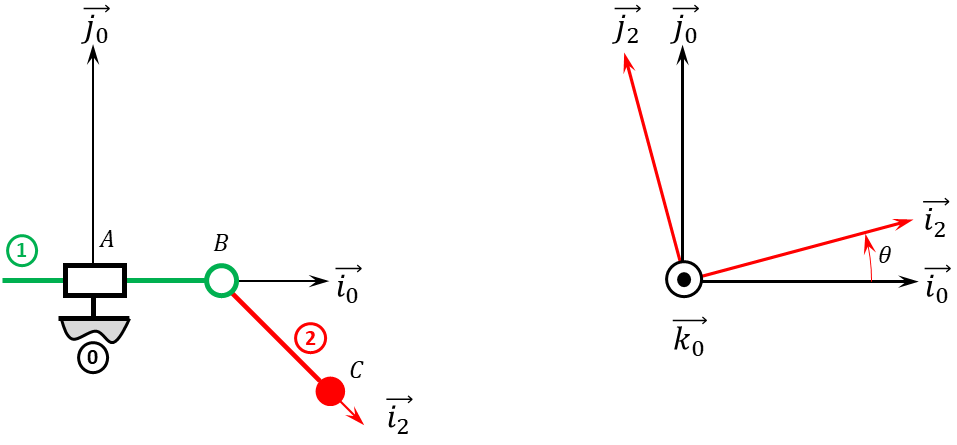
\includegraphics[width=\linewidth]{06_TR_01}
\end{center}
\fi

L'objectif est d'obtenir les lois de mouvement. 

\question{Appliquer le théorème du moment dynamique au solide \textbf{2} au point $B$ en projection sur $\vect{k_0}$.}
\ifprof
\begin{itemize}
\item \textbf{On isole 2.}
\item \textbf{BAME :}
\begin{itemize}
\item actions de la liaison pivot $\torseurstat{T}{1}{2}$; 
\item action de la pesanteur $\torseurstat{T}{\text{pes}}{2}$. On a $\vectm{B}{2}{0}\cdot \vect{k_0}=\vectm{G_2}{2}{0}\cdot \vect{k_0}+\left(\vect{BG_2}\wedge \left( -m_2 g \vj{0} \right) \right)\cdot \vect{k_0}$ $=\left(R\vi{2}\wedge \left( -m_2 g \vj{0} \right) \right)\cdot \vect{k_0}$
$=-m_2 g R  \vi{0}\cdot \vi{2} $ $=-m_2 g R  \cos\theta(t) $.
\end{itemize}
\item \textbf{Théorème :} on applique le théorème du moment dynamique en $B$ au solide \textbf{2} en projection sur $\vk{0}$ : $C_m+\vectm{B}{\text{pes}}{2}\cdot \vk{0}  = \vectmd{B}{2}{0}\cdot \vk{0}$.
On  a $ \vectmd{B}{2}{0}\cdot \vk{0}$ $=\left(C_1  \ddot{\theta} \vk{1} + R\left( -\sin \theta \ddot{\lambda}(t) \vk{0} 
+ R \ddot{\theta} \vk{2}\right) \right) \cdot \vk{0}$
 $=C_1  \ddot{\theta} + R\left( -\sin \theta \ddot{\lambda}(t) + R \ddot{\theta} \right)  $. Au final, 
 $ C_m-m_2 g R  \cos\theta(t) = C_1  \ddot{\theta} + R\left( -\sin \theta \ddot{\lambda}(t) + R \ddot{\theta} \right)$.
\end{itemize}




\else
\fi

\question{Appliquer le théorème de la résultante dynamique à l'ensemble \textbf{1+2} en projection sur $\vect{i_0}$}
\ifprof
\begin{itemize}
\item \textbf{On isole 1+2.}
\item \textbf{BAME :}
\begin{itemize}
\item actions de la liaison glissière $\torseurstat{T}{0}{1}$;
\item action de la pesanteur $\torseurstat{T}{\text{pes}}{1}$;
\item action de la pesanteur $\torseurstat{T}{\text{pes}}{2}$;
\item action du vérin $\torseurstat{T}{\text{ver}}{1}$.
\end{itemize}
\item \textbf{Théorème :} on applique le théorème de la résultante dynamique à l'ensemble \textbf{1+2} en projection sur 
$\vi{0}$ : 
$\vectf{\text{ver}}{1}\cdot \vi{0}  = \vectrd{1+2}{0}\cdot \vi{0}$. Au final, 
$F_{\text{ver}}=m_1\ddot{\lambda}(t)+m_2\left(\ddot{\lambda}(t)- R \left(\ddot{\theta} \sin\theta(t)  + \dot{\theta}^2 \cos\theta \right)\right)$.
\end{itemize}
\else
\fi

\ifprof
\else
\ifcolle
\else

\footnotesize
\begin{center}
\begin{tabular}{|p{.9\linewidth}|}
\hline
Indications :
\begin{enumerate}
\item $ C_m-m_2 g R  \cos\theta(t) = C_1  \ddot{\theta} + R\left( -\sin \theta \ddot{\lambda}(t) + R \ddot{\theta} \right)$;
\item $F_{\text{ver}}=m_1\ddot{\lambda}(t)+m_2\left(\ddot{\lambda}(t)- R \left(\ddot{\theta} \sin\theta(t)  + \dot{\theta}^2 \cos\theta \right)\right)$. 
\end{enumerate} \\ \hline
\end{tabular}
\end{center}
\normalsize
\fi

\begin{flushright}
\footnotesize{Corrigé  voir \ref{C2:09:06}.}
\end{flushright}%
\fi